\subsubsection{Brittle thrust wedges benchmark}
\label{sec:benchmark-brittle-thrust-wedge}

\textit{This section was contributed by Sibiao Liu, Stephanie Sparks, John
Naliboff, Cedric Thieulot, and Wolfgang Bangerth.}

Thrusting of brittle crust by applying compressive forces can lead to
large deformations. The process is complicated to model because the
rheology of cold, brittle crust is substantially more complicated than
that of the hot, ductile rocks in the mantle. At the same time, the
processes that act in such situations are surprisingly easy to
replicate and visualize using simple ``sand box'' experiments in which
one fills a volume with layers of differently-colored sand and compresses
or stretches the volume. Examples of the patterns one can then observe
in these do-it-yourself models are shown in
Fig.~\ref{fig:sandbox-images}.

\begin{figure}
  \centering
  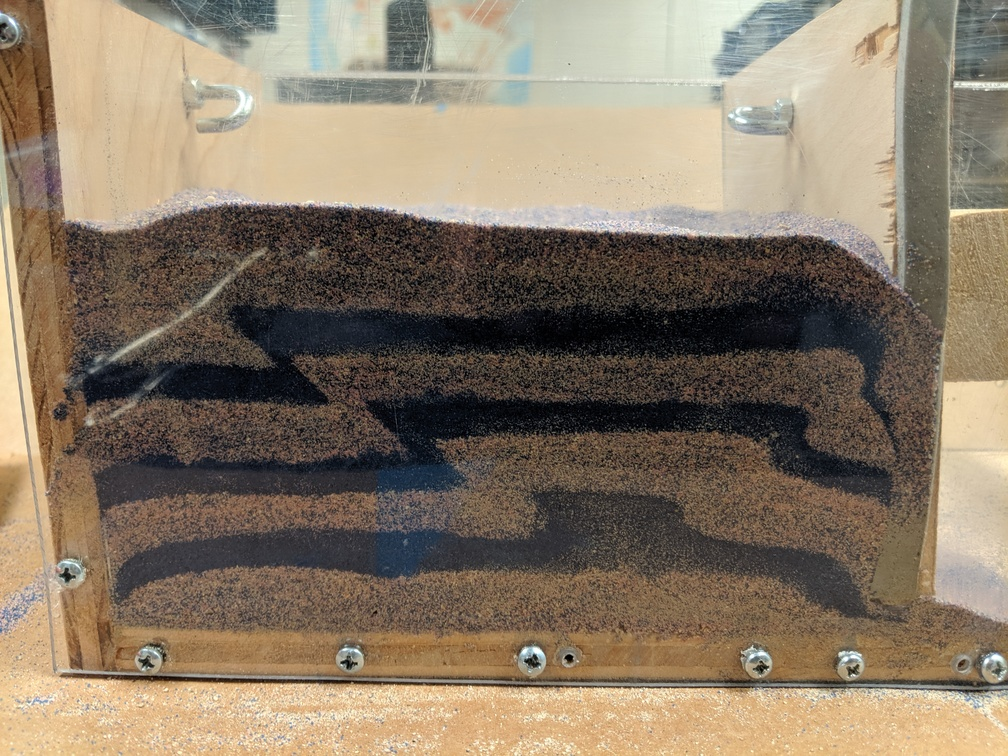
\includegraphics[width=0.45\textwidth]{cookbooks/benchmarks/buiter_et_al_2016_jsg/doc/real-sandbox-1.jpg}
  \hfill
  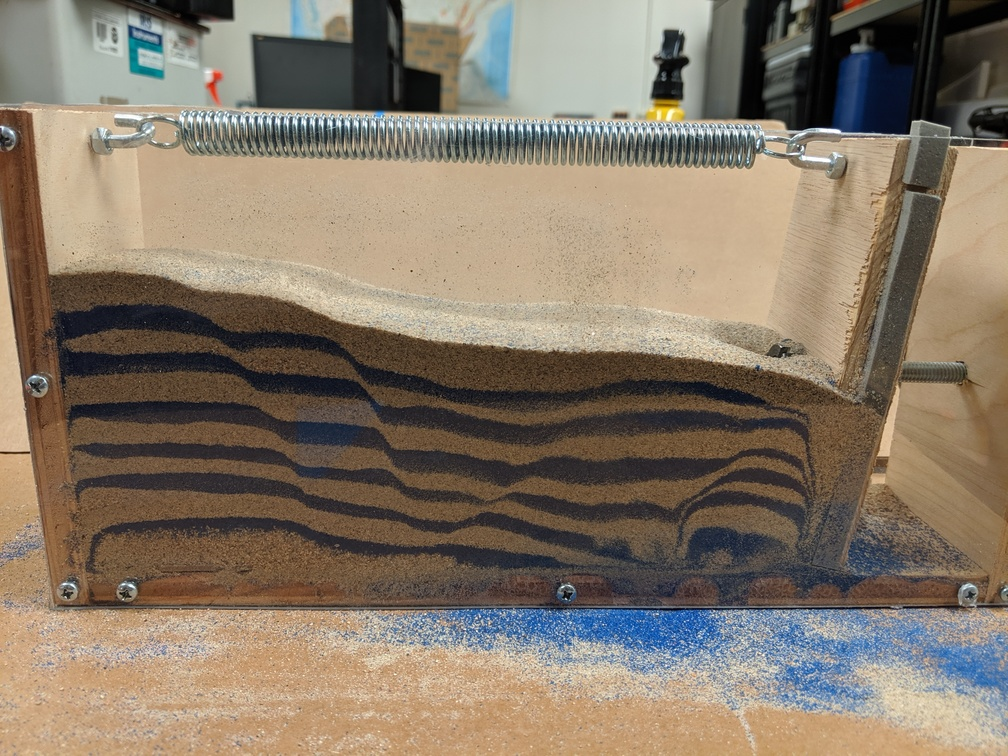
\includegraphics[width=0.45\textwidth]{cookbooks/benchmarks/buiter_et_al_2016_jsg/doc/real-sandbox-2.jpg}
  \caption{\it Examples of deformation patterns of ``sand box'' experiments in
    which alternating layers of differently-colored sand undergo deformation.
    Pictures courtesy of the lab of Dennis Harry at Colorado State University.}
  \label{fig:sandbox-images}
\end{figure}

Buiter et al.~\cite{buiter16} organized new comparison experiments between these kinds of
analogue and numerical models to investigate this kind of brittle thrust wedge behavior. The
benchmark here aims to verify that the wedge models using \aspect{} follows other
numerical results and the analytical wedge theory shown in this paper. In particular,
input files (\url{benchmarks/buiter_et_al_2016_jsg}) are provided for reproducing
the numerical simulations of stable wedge experiment 1 and unstable wedge experiment
2 with the same model setups.

A number of model sets of prescribed material behavior are required to simulate
the brittle thrust formation. For example, although the material in the numerical
model has a visco-plastic rheology, it performs plastic yielding at the beginning
of shortening due to the non-viscous sand. We prescribe plastic strain-weakening
behavior, with the internal angle of friction diminishing between total finite
strain invariant values of 0.5 and 1.0, to mimic the softening from peak to
dynamic stable strength which correlates with sand dilation.

In sandbox-type models, an important role is played by the boundaries and the
frictional sliding of sand against these boundaries. For the top boundary condition,
zero traction (``open'') and a sticky air layer is used to approximate a free surface.
Additional testing revealed that using a true free surface leads to significant
mesh distortion and associated numerical instabilities. We also apply a rigid block
that approximates a mobile wall with a constant velocity of 2.5 cm/hour on the
right-hand side boundary to drive the deformation in the sand layers. The following
listing shows key portions of the parameter file that describes this kind of setup:

\lstinputlisting[language=prmfile]{cookbooks/benchmarks/buiter_et_al_2016_jsg/doc/velocity_bc.part.prm}

Accurate solver convergence is always challenging to achieve in numerical thrust
wedge models with a high spatial resolution (ca. 1 mm node spacing) and a large
viscosity contrast. Here, we suggest that several parameters should be considered
carefully. First, the nonlinear and linear solver tolerances should be sufficiently
strict to avoid numerical instabilities. Second, we use the discontinuous Galerkin
method (\texttt{set Use discontinuous composition discretization = true}) to ensure
that the discontinuous composition bound preserving limiter produces sharp interfaces
between compositional layers. Lastly, we use the harmonic averaging scheme for
material and viscosity is required to achieve reasonable convergence behavior. The
relevant parameters are shown here:

\lstinputlisting[language=prmfile]{cookbooks/benchmarks/buiter_et_al_2016_jsg/doc/convergence.part.prm}

\textit{Experiment 1} tests whether model wedges in the stable domain of critical
taper theory remain stable when translated horizontally. A quartz sand wedge with
a horizontal base and a surface slope of 20 degrees is pushed 4 cm horizontally by
inward movement of a mobile wall at the right boundary with a velocity of 2.5 cm/hour
(Figure~\ref{fig:btwexp1}). The basal angle is zero (horizontal), a thin layer separates
the sand and boundary to ensure minimum coupling between the wedge and bounding box
during translation, and a sticky air layer is used above the wedge. Further, the purely
plastic material should not undergo any deformation during translation.

\begin{figure}
\begin{center}
  \centering
  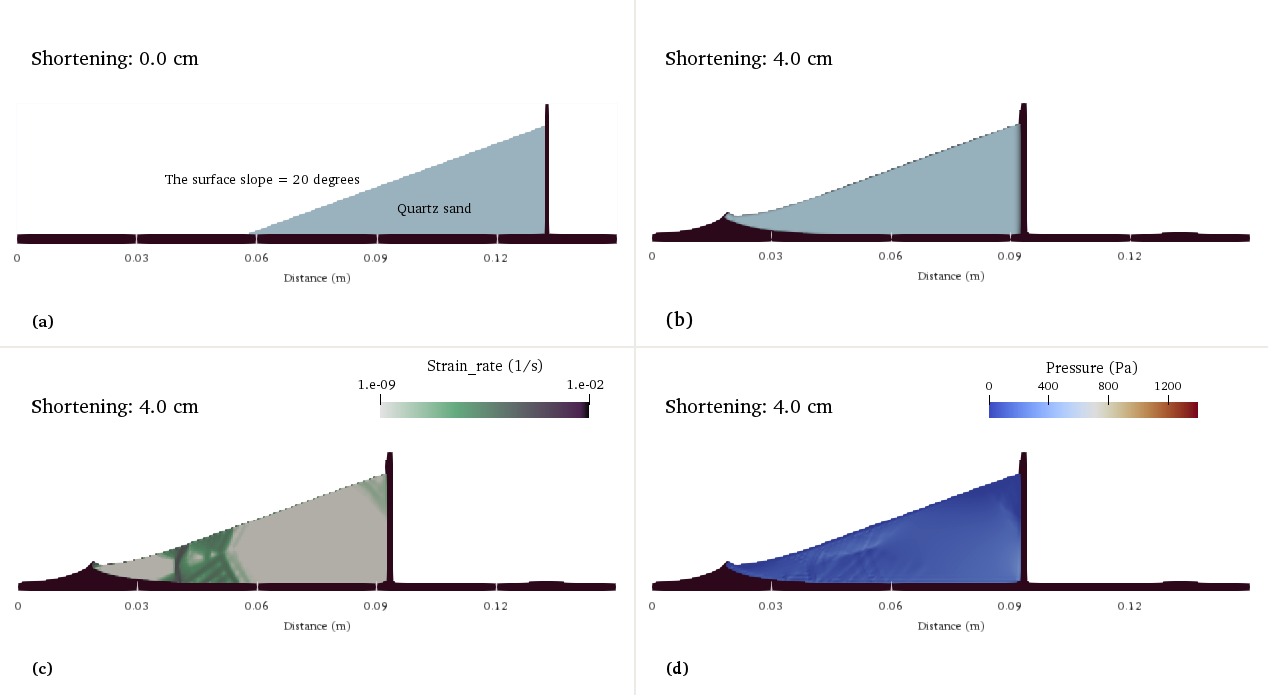
\includegraphics[width=\textwidth]{cookbooks/benchmarks/buiter_et_al_2016_jsg/doc/exp1.png}
  \caption{\it Numerical model of a stable sand wedge. a) Initial model setup. b) Material field after 4 cm of translation. c) Strain rate field and d) pressure field.}
  \label{fig:btwexp1}
\end{center}
\end{figure}

\textit{Experiment 2} tests how an unstable subcritical wedge deforms to reach the
critical taper solution. In this experiment, horizontal layers of sand undergo 10 cm
shortening by inward movement of a mobile wall with a velocity of 2.5 cm/hour
(Figure~\ref{fig:btwexp2}). Model results show thrust wedge generation near the
mobile wall through a combination of mainly in-sequence forward and backward thrusting.
The strain field highlights several incipient shear zones that do not always accumulate
enough offset to become visible in the material field. The pressure field of the model
remains more or less lithostatic, with lower pressure values in (incipient) shear zones.

\begin{figure}
\begin{center}
  \centering
  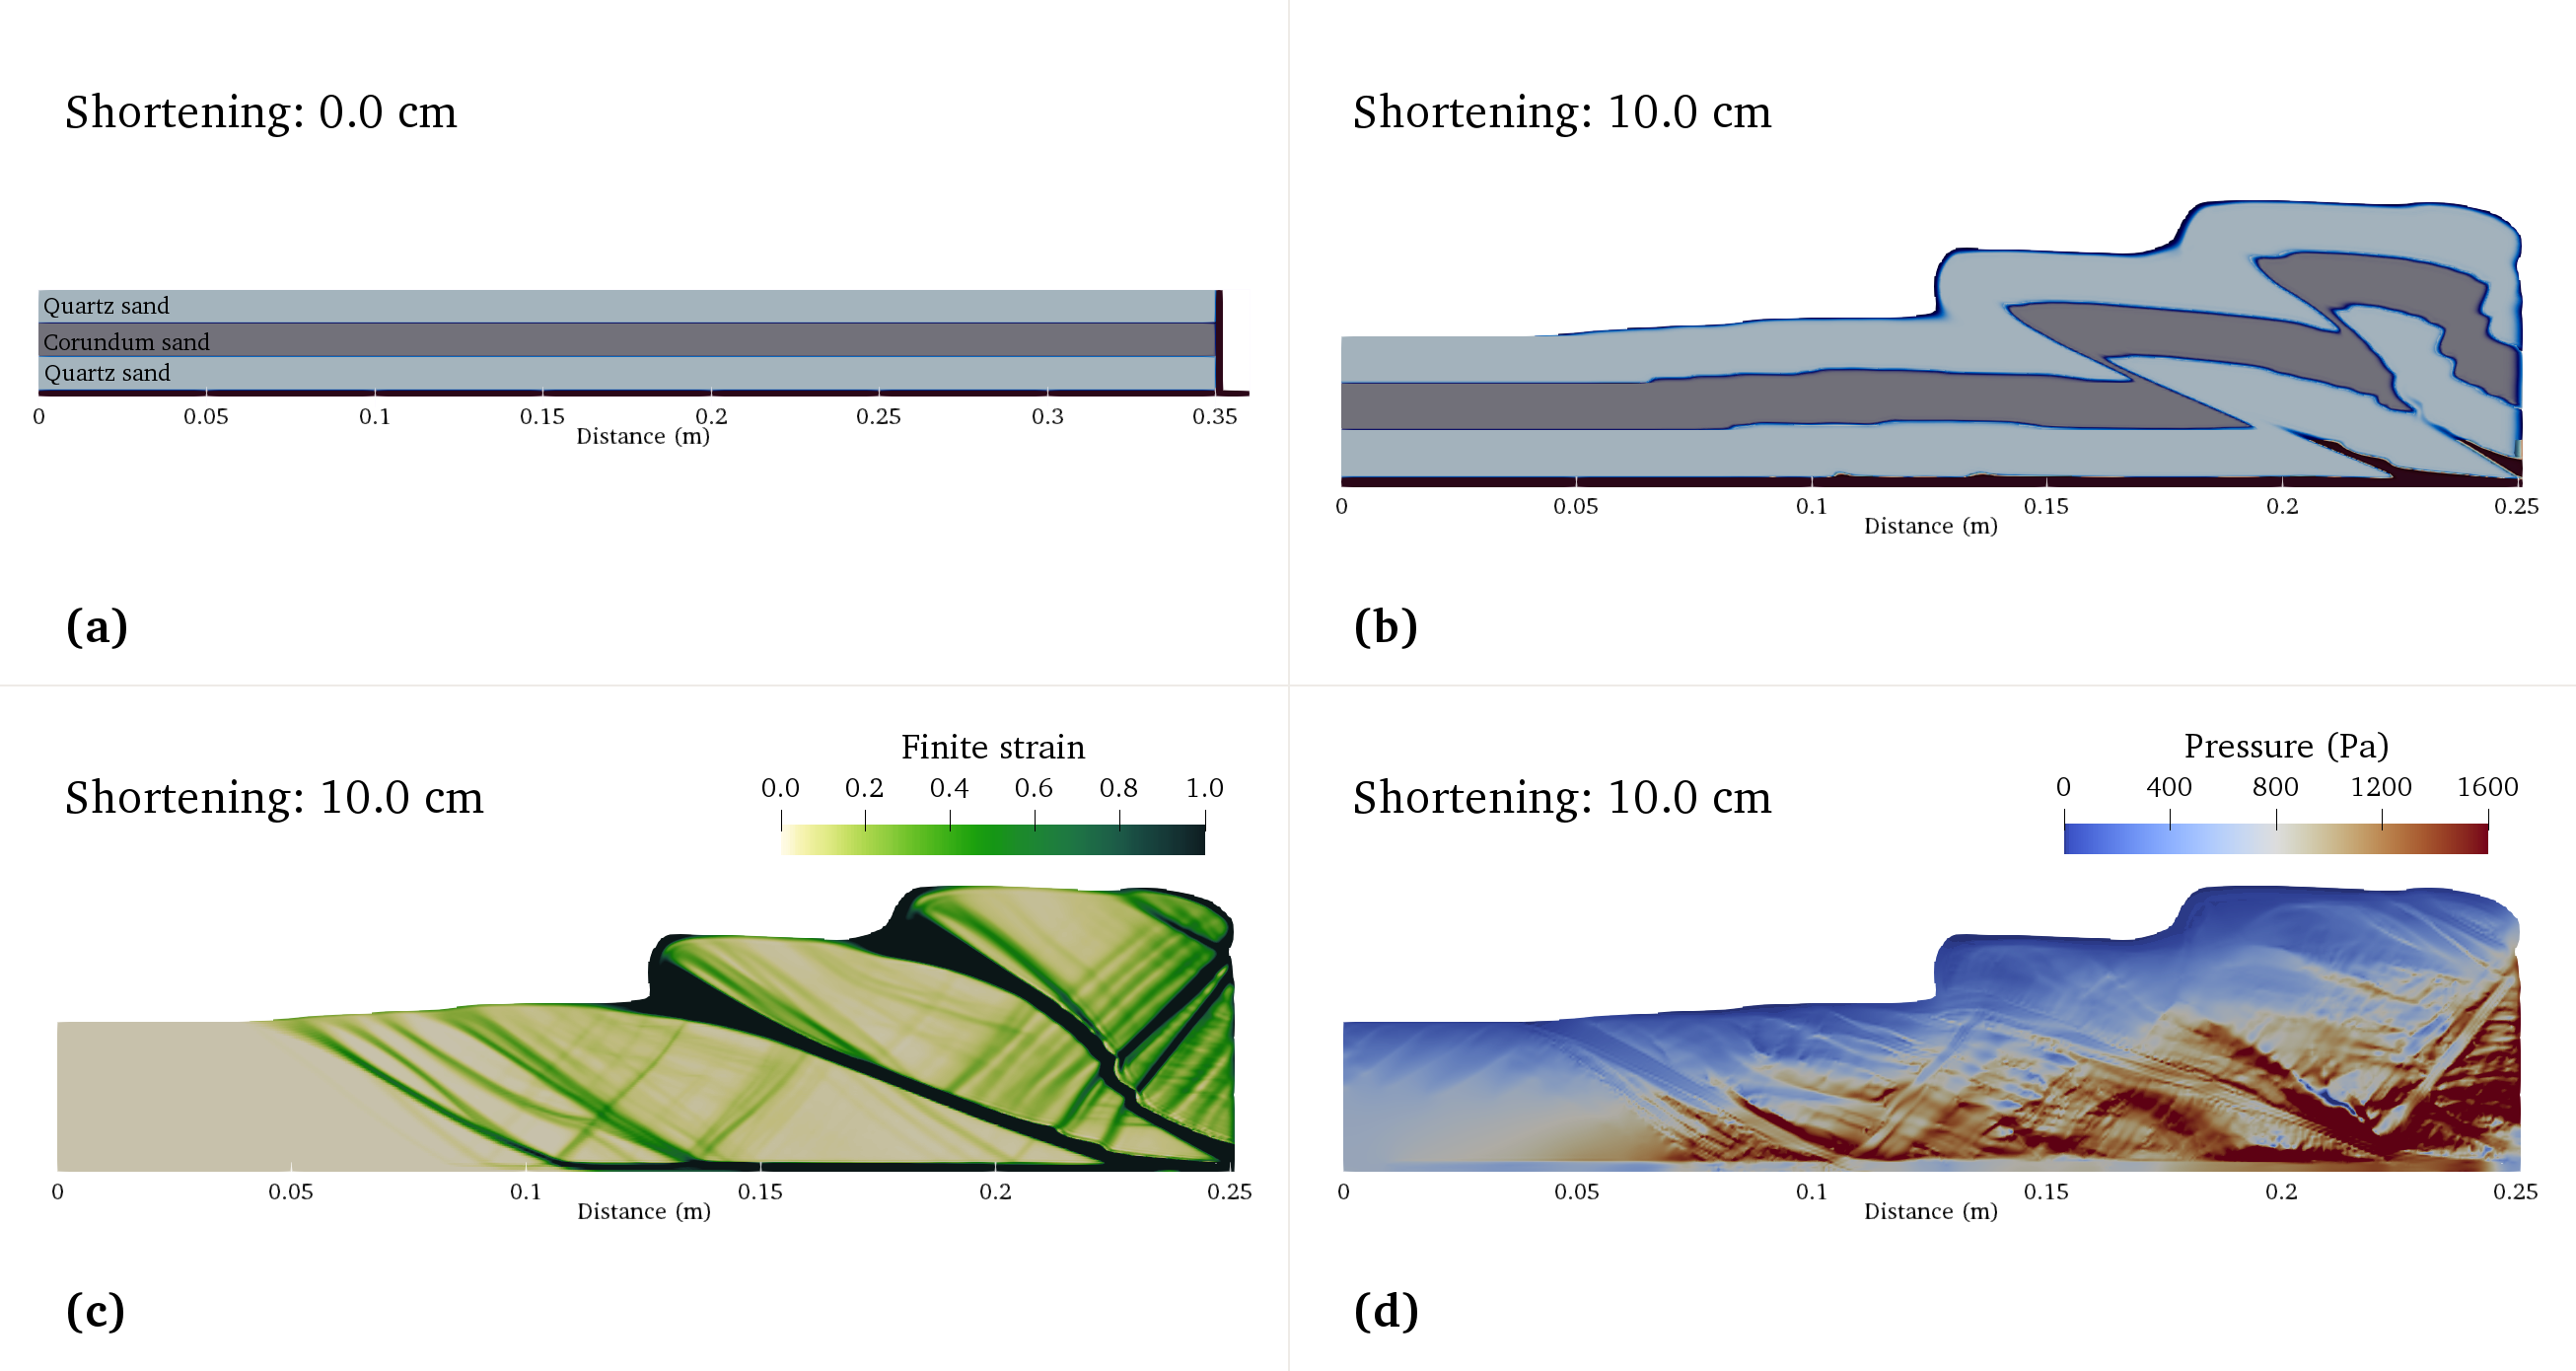
\includegraphics[width=\textwidth]{cookbooks/benchmarks/buiter_et_al_2016_jsg/doc/exp2.png}
  \caption{\it Numerical model of an unstable subcritical wedge. a) Initial model setup. b) Material field of sands after 10 cm shortening. c) Strain field and d) pressure field.}
  \label{fig:btwexp2}
\end{center}
\end{figure}
